\documentclass[12pt]{article}

%\usepackage{doublespace}
% or, get "double spacing" through:
% \renewcommand{\baselinestretch}{2}

\usepackage{graphicx}

\usepackage{fancyheadings}
\pagestyle{fancy}

% http://www.ctan.org/tex-archive/help/Catalogue/entries/syntax-mdw.html
\usepackage{syntax}
\grammarindent=3cm

% http://www.ccs.neu.edu/home/dorai/tex2page/tex2page-doc.html
\usepackage{tex2page}

% suppress "overfull" and "underfull" messages
%\tolerance=500

% 2 spaces after a period
\nonfrenchspacing

% 'sloppy' ensures everything falls within the margins,
% but the text spacing is distorted and looks, well, sloppy
%\sloppy

\newcommand{\greeke}{\ensuremath{\varepsilon}}%
\newcommand{\myref}[1][blah]{\ref{#1}}%


	\newif\ifpdf
	\ifx\pdfoutput\undefined
        \pdffalse
	\else
        \pdfoutput=1
        \pdftrue
    \fi
% Set up PDF specific
	\ifpdf
		\renewcommand\url\undefined % sorry, tex2page, hyperref provides its own
	    \usepackage[pdftex,colorlinks=true,urlcolor=blue,pdfstartview=FitH]{hyperref}
	    \pdfcompresslevel=9
		\DeclareGraphicsExtensions{.pdf}
	    \hypersetup{
			pdftitle={Implementing a Python to Scheme Compiler},
			pdfauthor={Daniel P.M. Silva}
	    }
	\else
%		\usepackage{hyperref}
	\fi


\hyphenation{Mz-Scheme}
\hyphenation{Dr-Scheme}
\hyphenation{Mr-Ed}


\title{Implementing a Python to Scheme Compiler}
\author{Daniel P.M. Silva}
\date{\today}

\begin{document}

	\maketitle
	\abstract{

This paper describes a Python-to-Scheme compiler.  The compiler translates Python code into its Scheme equivalent and provides a runtime system to model the Python environment.  The generated Scheme code may be evaluated or used by DrScheme tools, giving Python programmers access to the entire DrScheme suite while writing in their favorite language, and giving Scheme programmers access to Python libraries.

}
%	\section {Introduction}
%		\emph{Section omitted.}
	
\section{Introduction}

%With the availability of a Python-to-Scheme compiler, Python programmers can benefit from using the DrScheme suite to develop their code, as they will automatically inherit all the development tools provided with the IDE.  Scheme programmers are likely to benefit as well, considering they will be able to access the rich Python run-time system from their Scheme programs.

Programming languages are tools wielded by software developers.  This paper describes a compiler that translates one such language, Python, into another, MzScheme.  The translator allows Python developers to use PLT's software development tools and provides Scheme developers access to the rich Python runtime system.

  Section~\ref{background} will present the necessary background for the project, followed in Section~\ref{grammar} by the BNF grammar used by the compiler.  Finally, the fourth section will describe the current implementation of the compiler.


%	\section {Background}
%		\emph{Section omitted.}
	\section{Background}
\label{background}

The Python programming language~\cite{pythonlang} was designed by Guido van Rossum in the early 1990s as a descendant of the ABC programming language, which was a teaching language created by van Rossum in the early 1980s.  It includes a sizeable standard library, powerful primitive data types, and a self-documenting system based on the language's emphasis on readability of source text.  It is interpreted by a few different programs: C-Python~\cite{python}, currently the most widely used interpreter for the Python programming language, is implemented in the C language.  Another Python interpreter, Jython~\cite{jython}, is written in Java.  The compiler this paper describes serves as yet another interpreter; it is written in MzScheme.

MzScheme~\cite{mzscheme} is an interpreter for the MzScheme programming language~\cite{mzschemelang}, which is a dialect of the Scheme language~\cite{kelsey98revised}.  MzScheme compiles syntactically valid MzScheme language programs into the MzScheme Core language, a subset of the MzScheme language, before compiling the core language into an internal bytecode representation for evaluation.

MrEd~\cite{mred} is a graphical user interface (GUI) toolkit that builds on the MzScheme interpreter and works uniformally across several platforms, namely Windows, Mac OS X, and the X Window System.

\begin{figure}
	\caption{PLT Scheme partial language hierarchy}
	\label{schemelanguagesfig}
	\begin{center}
		\includegraphics{images/scheme-languages}
	\end{center}
\end{figure}


Originally meant for Scheme, DrScheme~\cite{bruce97drscheme} is an integrated development environment (IDE) based on MzScheme---it is a MrEd application---with support for embedding third-party extensions.  DrScheme provides developers with useful and modular development tools, such as syntax or flow analyzers, which accept the MzScheme Core language as their input.  Because the internal DrScheme data structures representing MzScheme code also store source file location, any reference by a development tool or the MzScheme interpreter to the Core code can be mapped back to a reference to the original program text.

DrScheme is no longer a development environment only for Scheme.  It can now potentially play the role of a program development environment for any language, which users can select from a menu (Figure~\ref{drschemelangmenufig}).  When using any language from within the IDE, the program developer may use all of DrScheme's development tools, such as Syntax Check, which checks a program's syntax and highlights its bindings (Figure~\ref{syntaxcheckschemefig}), or MrFlow, which analyses a program's possible flow of values.  Also, any new tool added to the DrScheme IDE will automatically work with all languages that DrScheme now supports (Figure~\ref{syntaxcheckpythonfig}).

\begin{figure}
	\caption{DrScheme language selection menu}
	\label{drschemelangmenufig}
	\begin{center}
		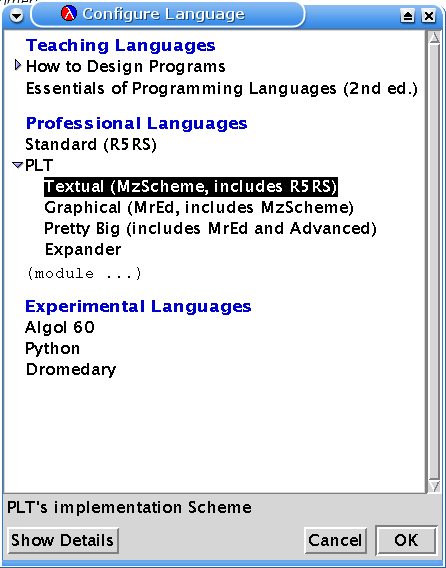
\includegraphics{images/drscheme-lang-menu}
	\end{center}
\end{figure}

To support a new language, however, DrScheme needs software to translate programs written in the new language into MzScheme.  In the case of adding Python support to DrScheme, this is the task of the Python-to-Scheme compiler.  The compiler is packaged as a DrScheme language tool, thus introducing Python as a language in DrScheme's graphical list of choices (Figure~\ref{drschemelangmenufig}).  This paper describes the components that comprise the compiler.  Section~\ref{grammar} presents the Python grammar used in this implementation.  Section~\ref{implementation} describes the implementation itself.

\begin{figure}
	\caption{Syntax Check and Scheme}
	\label{syntaxcheckschemefig}
	\begin{center}
		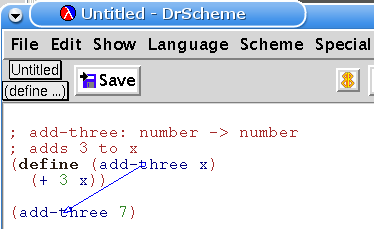
\includegraphics{images/syntax-check-scheme}
	\end{center}
\end{figure}

\begin{figure}
	\caption{Syntax Check and Python}
	\label{syntaxcheckpythonfig}
	\begin{center}
		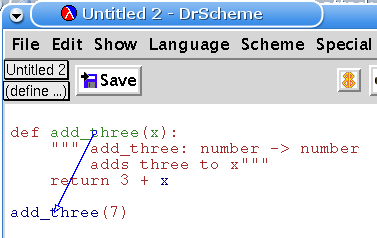
\includegraphics{images/syntax-check-python}
	\end{center}
\end{figure}


	\let\rulesection\subsubsection
	\section{Grammar}
		\label{grammar}
%		\emph{Section omitted.}
		This section presents the grammar for Python programs currently supported by the Python-to-Scheme compiler.

The starting non-terminal is usually \synt{file_input} (\ref{filezzzinputb}), but \linebreak[4] \synt{eval_input} (\ref{evalzzzinputb}) is used instead by the \verb|eval| function.

If a non-terminal is named \synt{nonterm_list_plus}, it is assumed that it defines the regular expression \emph{nonterm+}, while \synt{nonterm_list} usually defines the regular expression \emph{nonterm*}, though it might be \emph{(nonterm ,)*} as well.

The empty string is represented by \greeke{}.
		\subsection{Program}
			% Program rules

\rulesection{file\_input}
\label{filezzzinputb}
This non-terminal is the result of the parser in the following situations:
\begin{itemize}
\item when parsing a complete Python program (from a file or from a string);
\item when parsing a module;
\item when parsing a string passed to the exec statement.
\end{itemize}

\begin{tabular}{lcl}
{\bf \verb+<+file\_input\verb+>+} & ::=  & $\varepsilon$ \\
 & \verb+|+  & {\bf \verb+<+file\_input~\ref{filezzzinputb}\verb+>+}  NEWLINE \\
 & \verb+|+  & {\bf \verb+<+file\_input~\ref{filezzzinputb}\verb+>+}  {\bf \verb+<+stmt~\ref{stmtb}\verb+>+}  \\
\end{tabular}

\rulesection{eval\_input}
\label{evalzzzinputb}
Eval Input is used by the Python \verb+eval+ and \verb+input+ functions.  Only expressions (\ref{tuplezzzorzzztestb}), possibly followed by newlines, are allowed. \\

\begin{tabular}{lcl}
{\bf \verb+<+eval\_input\verb+>+} & ::=  & {\bf \verb+<+tuple\_or\_test~\ref{tuplezzzorzzztestb}\verb+>+}  \\
 & \verb+|+  & {\bf \verb+<+eval\_input~\ref{evalzzzinputb}\verb+>+}  NEWLINE \\
\end{tabular}


		\subsection{Statements}
			% Statement rules
\newlength{\tw}
\newlength{\len}

\rulesection{stmt}
\label{stmtb}

\begin{grammar}
<stmt> ::= <simple_stmt \myref[simplezzzstmtb]>
	\alt <compound_stmt \myref[compoundzzzstmtb]>
\end{grammar}
%\begin{tabular}{lcl}
%{\bf \verb+<+stmt\verb+>+} & ::=  & {\bf \verb+<+simple\_stmt~\ref{simplezzzstmtb}\verb+>+}  \\
% & \verb+|+  & {\bf \verb+<+compound\_stmt~\ref{compoundzzzstmtb}\verb+>+}  \\
%\end{tabular} \\

Simple statements (\ref{simplezzzstmtb}) span a single line (no new indentation levels).  Compound statements (\ref{compoundzzzstmtb}) may span multiple lines. \\

\rulesection{simple\_stmt}
\label{simplezzzstmtb}

\begin{grammar}
<simple_stmt> ::= <small_stmt \myref[smallzzzstmtb]> NEWLINE
	\alt <small_stmt \myref[smallzzzstmtb]> `;' NEWLINE
	\alt <small_stmt \myref[smallzzzstmtb]> `;' <simple_stmt>
\end{grammar}

%\begin{tabular}{lcl}
%{\bf \verb+<+simple\_stmt\verb+>+} & ::=  & {\bf \verb+<+small\_stmt~\ref{smallzzzstmtb}\verb+>+}  NEWLINE \\
% & \verb+|+  & {\bf \verb+<+small\_stmt~\ref{smallzzzstmtb}\verb+>+}  \verb|;| NEWLINE \\
% & \verb+|+  & {\bf \verb+<+small\_stmt~\ref{smallzzzstmtb}\verb+>+}  \verb|;| {\bf %\verb+<+simple\_stmt~\ref{simplezzzstmtb}\verb+>+}  \\
%\end{tabular}

\rulesection{small\_stmt}
\label{smallzzzstmtb}

\begin{grammar}
<small_stmt> ::= <expr_stmt \myref[exprzzzstmtb]>
	\alt <print_stmt \myref[printzzzstmtb]>
	\alt <del_stmt \myref[delzzzstmtb]>
	\alt <pass_stmt \myref[passzzzstmtb]>
	\alt <flow_stmt \myref[flowzzzstmtb]>
	\alt <import_stmt \myref[importzzzstmtb]>
	\alt <global_stmt \myref[globalzzzstmtb]>
	\alt <exec_stmt \myref[execzzzstmtb]>
	\alt <assert_stmt \myref[assertzzzstmtb]>
\end{grammar}

%\begin{tabular}{lcl}
%{\bf \verb+<+small\_stmt\verb+>+} & ::=  & {\bf \verb+<+expr\_stmt~\ref{exprzzzstmtb}\verb+>+}  \\
% & \verb+|+  & {\bf \verb+<+print\_stmt~\ref{printzzzstmtb}\verb+>+}  \\
% & \verb+|+  & {\bf \verb+<+del\_stmt~\ref{delzzzstmtb}\verb+>+}  \\
% & \verb+|+  & {\bf \verb+<+pass\_stmt~\ref{passzzzstmtb}\verb+>+}  \\
% & \verb+|+  & {\bf \verb+<+flow\_stmt~\ref{flowzzzstmtb}\verb+>+}  \\
% & \verb+|+  & {\bf \verb+<+import\_stmt~\ref{importzzzstmtb}\verb+>+}  \\
% & \verb+|+  & {\bf \verb+<+global\_stmt~\ref{globalzzzstmtb}\verb+>+}  \\
% & \verb+|+  & {\bf \verb+<+exec\_stmt~\ref{execzzzstmtb}\verb+>+}  \\
% & \verb+|+  & {\bf \verb+<+assert\_stmt~\ref{assertzzzstmtb}\verb+>+}  \\
%\end{tabular}

\rulesection{expr\_stmt}
\label{exprzzzstmtb}

\begin{grammar}
<expr_stmt> ::= <test \myref[testb]> <augassign \myref[augassignb]> <tuple_or_test \myref[tuplezzzorzzztestb]>
	\alt <testlist_list_plus \myref[testlistzzzlistzzzplusb]>
\end{grammar}

%\begin{tabular}{lcl}
%{\bf \verb+<+expr\_stmt\verb+>+} & ::=  & {\bf \verb+<+test~\ref{testb}\verb+>+}  {\bf \verb+<+augassign~\ref{augassignb}\verb+>+}  {\bf \verb+<+tuple\_or\_test~\ref{tuplezzzorzzztestb}\verb+>+}  \\
% & \verb+|+  & {\bf \verb+<+testlist\_list\_plus~\ref{testlistzzzlistzzzplusb}\verb+>+}  \\
%\end{tabular} \\

An expression statement consists of either a mutative operation or a \synt{testlist_list_plus} (\ref{testlistzzzlistzzzplusb}). %{\bf \verb+<+testlist\_list\_plus~\ref{testlistzzzlistzzzplusb}\verb+>+}.

\rulesection{testlist\_list\_plus}
\label{testlistzzzlistzzzplusb}

\begin{grammar}
<testlist_list_plus> ::= <tuple_or_test \myref[tuplezzzorzzztestb]>
	\alt <tuple_or_test \myref[tuplezzzorzzztestb]> `=' <testlist_list_plus>
\end{grammar}

%\begin{tabular}{lcl}
%{\bf \verb+<+testlist\_list\_plus\verb+>+} & ::=  & {\bf \verb+<+tuple\_or\_test~\ref{tuplezzzorzzztestb}\verb+>+}  \\
% & \verb+|+  & {\bf \verb+<+tuple\_or\_test~\ref{tuplezzzorzzztestb}\verb+>+}  \verb|=| {\bf \verb+<+testlist\_list\_plus~\ref{testlistzzzlistzzzplusb}\verb+>+}  \\
%\end{tabular} \\

A \synt{testlist_list_plus} is an assignment or an expression (\ref{tuplezzzorzzztestb}) which will be displayed in the output of the interpreter.

\rulesection{augassign}
\label{augassignb}

\begin{grammar}
<augassign> ::= `+='
	\alt `-='
	\alt `*='
	\alt `/='
	\alt `%='
	\alt `&='
	\alt `|='
	\alt `^='
	\alt `<<='
	\alt `>>='
	\alt `**='
	\alt `//='
\end{grammar}

%\begin{tabular}{lcl}
%{\bf \verb+<+augassign\verb+>+} & ::=  & \verb|+=| \\
% & \verb+|+  & \verb|-=| \\
% & \verb+|+  & \verb|*=| \\
% & \verb+|+  & \verb|/=| \\
% & \verb+|+  & \verb|%=| \\
% & \verb+|+  & \verb|&=| \\
% & \verb+|+  & \verb+|=+ \\
% & \verb+|+  & \verb|^=| \\
% & \verb+|+  & \verb|<<=| \\
% & \verb+|+  & \verb|>>=| \\
% & \verb+|+  & \verb|**=| \\
% & \verb+|+  & \verb|//=| \\
%\end{tabular}

\rulesection{print\_stmt}
\label{printzzzstmtb}

\begin{grammar}
<print_stmt> ::= `print' <test_list \myref[testzzzlistb]>
	\alt `print' `>>' <test_list \myref[testzzzlistb]>
\end{grammar}

%\begin{tabular}{lcl}
%{\bf \verb+<+print\_stmt\verb+>+} & ::=  & print {\bf \verb+<+test\_list~\ref{testzzzlistb}\verb+>+}  \\
% & \verb+|+  & print \verb|>>| {\bf \verb+<+test\_list~\ref{testzzzlistb}\verb+>+}  \\
%\end{tabular} \\

From the Python Reference~\cite{pythonlang}, section 6.6:
\begin{quote}
\verb|print| has an extended form, sometimes referred to as ``print chevron.'' 
In this form, the first expression after the \verb+>>+ must evaluate to a ``file-like'' 
object, specifically an object that has a \verb|write| method, or \verb|None|.
\end{quote}

\rulesection{del\_stmt}
\label{delzzzstmtb}
See the Python Reference~\cite{pythonlang}, section 6.5.

\begin{grammar}
<del_stmt> ::= `del' <target_tuple_or_expr \myref[targetzzztuplezzzorzzzexprb]>
\end{grammar}

%\begin{tabular}{lcl}
%{\bf \verb+<+del\_stmt\verb+>+} & ::=  & del {\bf \verb+<+target\_tuple\_or\_expr~\ref{targetzzztuplezzzorzzzexprb}\verb+>+}  \\
%\end{tabular}

\rulesection{pass\_stmt}
\label{passzzzstmtb}

\begin{grammar}
<pass_stmt> ::= `pass'
\end{grammar}

%\begin{tabular}{lcl}
%{\bf \verb+<+pass\_stmt\verb+>+} & ::=  & pass \\
%\end{tabular}

\rulesection{flow\_stmt}
\label{flowzzzstmtb}
A flow statement directs or modifies program flow. \\

\begin{grammar}
<flow_stmt> ::= <break_stmt \myref[breakzzzstmtb]>
	\alt <continue_stmt \myref[continuezzzstmtb]>
	\alt <return_stmt \myref[returnzzzstmtb]>
	\alt <raise_stmt \myref[raisezzzstmtb]>
	\alt <yield_stmt \myref[yieldzzzstmtb]>
\end{grammar}

%\begin{tabular}{lcl}
%{\bf \verb+<+flow\_stmt\verb+>+} & ::=  & {\bf \verb+<+break\_stmt~\ref{breakzzzstmtb}\verb+>+}  \\
% & \verb+|+  & {\bf \verb+<+continue\_stmt~\ref{continuezzzstmtb}\verb+>+}  \\
% & \verb+|+  & {\bf \verb+<+return\_stmt~\ref{returnzzzstmtb}\verb+>+}  \\
% & \verb+|+  & {\bf \verb+<+raise\_stmt~\ref{raisezzzstmtb}\verb+>+}  \\
% & \verb+|+  & {\bf \verb+<+yield\_stmt~\ref{yieldzzzstmtb}\verb+>+}  \\
%\end{tabular}

\rulesection{break\_stmt}
\label{breakzzzstmtb}

\begin{grammar}
<break_stmt> ::= `break'
\end{grammar}

%\begin{tabular}{lcl}
%{\bf \verb+<+break\_stmt\verb+>+} & ::=  & break \\
%\end{tabular} \\

From the Python reference~\cite{pythonlang}, section 6.10:
\begin{quote}
\verb+break+ may only occur syntactically nested in a for or while loop, 
but not nested in a function or class definition within that loop.
\end{quote}

\rulesection{continue\_stmt}
\label{continuezzzstmtb}

\begin{grammar}
<continue_stmt> ::= `continue'
\end{grammar}

%\begin{tabular}{lcl}
%{\bf \verb+<+continue\_stmt\verb+>+} & ::=  & continue \\
%\end{tabular} \\

From the Python reference~\cite{pythonlang}, section 6.11:
\begin{quote}
\verb|continue| may only occur syntactically nested in a for or while loop, 
but not nested in a function or class definition or try statement within 
that loop.
\end{quote}

\rulesection{return\_stmt}
\label{returnzzzstmtb}

\begin{grammar}
<return_stmt> ::= `return' <tuple_or_test \myref[tuplezzzorzzztestb]>
	\alt `return'
\end{grammar}

%\begin{tabular}{lcl}
%{\bf \verb+<+return\_stmt\verb+>+} & ::=  & return {\bf \verb+<+tuple\_or\_test~\ref{tuplezzzorzzztestb}\verb+>+}  \\
% & \verb+|+  & return \\
%\end{tabular} \\

From the Python reference~\cite{pythonlang}, section 6.7:
\begin{quote}
In a generator function (see \ref{yieldzzzstmtb}), 
the \verb|return| statement is not allowed to include an expression list (\ref{tuplezzzorzzztestb}). In that context, a bare return indicates that the generator is done and will cause \verb|StopIteration| to be raised.
\end{quote}

\rulesection{raise\_stmt}
\label{raisezzzstmtb}

\begin{grammar}
<raise_stmt> ::= `raise'
	\alt `raise' <test \myref[testb]>
	\alt `raise' <test \myref[testb]> `,' <test \myref[testb]>
	\alt `raise' <test \myref[testb]> `,' <test \myref[testb]> `,' <test \myref[testb]>
\end{grammar}

%\begin{tabular}{lcl}
%{\bf \verb+<+raise\_stmt\verb+>+} & ::=  & raise \\
% & \verb+|+  & raise {\bf \verb+<+test~\ref{testb}\verb+>+}  \\
% & \verb+|+  & raise {\bf \verb+<+test~\ref{testb}\verb+>+}  \verb|,| {\bf \verb+<+test~\ref{testb}\verb+>+}  \\
% & \verb+|+  & raise {\bf \verb+<+test~\ref{testb}\verb+>+}  \verb|,| {\bf \verb+<+test~\ref{testb}\verb+>+}  \verb|,| {\bf \verb+<+test~\ref{testb}\verb+>+}  \\
%\end{tabular} \\

From the Python reference~\cite{pythonlang}, section 6.9:
\begin{quote}
\verb|raise| may have up to three arguments, the first being the type of the exception,
the second being its value, and the third being a traceback.
\end{quote}

\rulesection{yield\_stmt (NOT YET IMPLEMENTED)}
\label{yieldzzzstmtb}

\begin{grammar}
<yield_stmt> ::= `yield' <tuple_or_test \myref[tuplezzzorzzztestb]>
\end{grammar}

%\begin{tabular}{lcl}
%{\bf \verb+<+yield\_stmt\verb+>+} & ::=  & yield {\bf \verb+<+tuple\_or\_test~\ref{tuplezzzorzzztestb}\verb+>+}  \\
%\end{tabular} \\

From the Python reference~\cite{pythonlang}, section 6.8:
\begin{quote}
The \verb|yield| statement is only used when defining a generator function, 
and is only used in the body of the generator function. Using a yield 
statement in a function definition is sufficient to cause that definition 
to create a generator function instead of a normal function.
\end{quote}

\rulesection{import\_stmt}
\label{importzzzstmtb}

\begin{grammar}
<import_stmt> ::= <import_stmt1 \myref[importzzzstmt1b]>
	\alt `from' <dotted_name \myref[dottedzzznameb]> `import' `*'
	\alt `from' <dotted_name \myref[dottedzzznameb]> `import' <import_stmt2 \myref[importzzzstmt2b]>
\end{grammar}

%\begin{tabular}{lcl}
%{\bf \verb+<+import\_stmt\verb+>+} & ::=  & {\bf \verb+<+import\_stmt1~\ref{importzzzstmt1b}\verb+>+}  \\
% & \verb+|+  & from {\bf \verb+<+dotted\_name~\ref{dottedzzznameb}\verb+>+}  import \verb|*| \\
% & \verb+|+  & from {\bf \verb+<+dotted\_name~\ref{dottedzzznameb}\verb+>+}  import {\bf \verb+<+import\_stmt2~\ref{importzzzstmt2b}\verb+>+}  \\
%\end{tabular} \\

See the Python reference~\cite{pythonlang}, section 6.12.

\rulesection{import\_stmt1}
\label{importzzzstmt1b}

\begin{grammar}
<import_stmt1> ::= `import' <dotted_as_name \myref[dottedzzzaszzznameb]>
	\alt <import_stmt1> `,' <dotted_as_name \myref[dottedzzzaszzznameb]>
\end{grammar}

%\begin{tabular}{lcl}
%{\bf \verb+<+import\_stmt1\verb+>+} & ::=  & import {\bf \verb+<+dotted\_as\_name~\ref{dottedzzzaszzznameb}\verb+>+}  \\
% & \verb+|+  & {\bf \verb+<+import\_stmt1~\ref{importzzzstmt1b}\verb+>+}  \verb|,| {\bf \verb+<+dotted\_as\_name~\ref{dottedzzzaszzznameb}\verb+>+}  \\
%\end{tabular}

\rulesection{import\_stmt2}
\label{importzzzstmt2b}

\begin{grammar}
<import_stmt2> ::= <import_as_name \myref[importzzzaszzznameb]>
	\alt <import_as_name \myref[importzzzaszzznameb]> `,' <import_stmt2>
\end{grammar}

%\begin{tabular}{lcl}
%{\bf \verb+<+import\_stmt2\verb+>+} & ::=  & {\bf \verb+<+import\_as\_name~\ref{importzzzaszzznameb}\verb+>+}  \\
% & \verb+|+  & {\bf \verb+<+import\_as\_name~\ref{importzzzaszzznameb}\verb+>+}  \verb|,| {\bf \verb+<+import\_stmt2~\ref{importzzzstmt2b}\verb+>+}  \\
%\end{tabular}

\rulesection{import\_as\_name}
\label{importzzzaszzznameb}

\begin{grammar}
<import_as_name> ::= <ident \myref[identb]> NAME <ident \myref[identb]>
	\alt <ident \myref[identb]>
\end{grammar}

%\begin{tabular}{lcl}
%{\bf \verb+<+import\_as\_name\verb+>+} & ::=  & {\bf \verb+<+ident~\ref{identb}\verb+>+}  NAME {\bf \verb+<+ident~\ref{identb}\verb+>+}  \\
% & \verb+|+  & {\bf \verb+<+ident~\ref{identb}\verb+>+}  \\
%\end{tabular}

\rulesection{dotted\_as\_name}
\label{dottedzzzaszzznameb}

\begin{grammar}
<dotted_as_name> ::= <dotted_name \myref[dottedzzznameb]> NAME <ident \myref[identb]>
	\alt <dotted_name \myref[dottedzzznameb]>
\end{grammar}

%\begin{tabular}{lcl}
%{\bf \verb+<+dotted\_as\_name\verb+>+} & ::=  & {\bf \verb+<+dotted\_name~\ref{dottedzzznameb}\verb+>+}  NAME {\bf \verb+<+ident~\ref{identb}\verb+>+}  \\
% & \verb+|+  & {\bf \verb+<+dotted\_name~\ref{dottedzzznameb}\verb+>+}  \\
%\end{tabular}

\rulesection{dotted\_name}
\label{dottedzzznameb}

\begin{grammar}
<dotted_name> ::= <ident \myref[identb]>
	\alt <ident \myref[identb]> `.' <dotted_name>
\end{grammar}

%\begin{tabular}{lcl}
%{\bf \verb+<+dotted\_name\verb+>+} & ::=  & {\bf \verb+<+ident~\ref{identb}\verb+>+}  \\
% & \verb+|+  & {\bf \verb+<+ident~\ref{identb}\verb+>+}  \verb|.| {\bf \verb+<+dotted\_name~\ref{dottedzzznameb}\verb+>+}  \\
%\end{tabular}

\rulesection{global\_stmt}
\label{globalzzzstmtb}

\begin{grammar}
<global_stmt> ::= `global' <ident \myref[identb]>
	\alt <global_stmt \myref[globalzzzstmtb]> `,' <ident \myref[identb]>
\end{grammar}

%\begin{tabular}{lcl}
%{\bf \verb+<+global\_stmt\verb+>+} & ::=  & global {\bf \verb+<+ident~\ref{identb}\verb+>+}  \\
% & \verb+|+  & {\bf \verb+<+global\_stmt~\ref{globalzzzstmtb}\verb+>+}  \verb|,| {\bf \verb+<+ident~\ref{identb}\verb+>+}  \\
%\end{tabular} \\

From the Python reference~\cite{pythonlang}, section 6.13:
\begin{quote}
The global statement means that the listed identifiers are to be interpreted as globals.
Names listed in a global statement must not be used in the same code block 
textually preceding that global statement (not yet implemented). Names listed in a global statement must not be defined as formal parameters or in a for loop control target, class definition, function definition, or import statement (not yet implemented).

Programmer's note: the global is a directive to the parser. 
It applies only to code parsed at the same time as the global statement. 
In particular, a global statement contained in an exec statement does not 
affect the code block containing the exec statement, and code contained in 
an exec statement is unaffected by global statements in the code containing 
the exec statement. The same applies to the eval(), execfile() and compile() 
functions.

For example, in:
\begin{verbatim}
exec "global x"
x = 2
\end{verbatim}
the generated code will define a new \verb|x|, not modify an existing one.
\end{quote}

\rulesection{exec\_stmt (NOT YET IMPLEMENTED)}
\label{execzzzstmtb}

\begin{grammar}
<exec_stmt> ::= `exec' <expr \myref[exprb]>
	\alt `exec' <expr \myref[exprb]> `in' <test \myref[testb]>
	\alt `exec' <expr \myref[exprb]> `in' <test \myref[testb]> `,' <test \myref[testb]>
\end{grammar}

%\begin{tabular}{lcl}
%{\bf \verb+<+exec\_stmt\verb+>+} & ::=  & exec {\bf \verb+<+expr~\ref{exprb}\verb+>+}  \\
% & \verb+|+  & exec {\bf \verb+<+expr~\ref{exprb}\verb+>+}  in {\bf \verb+<+test~\ref{testb}\verb+>+}  \\
% & \verb+|+  & exec {\bf \verb+<+expr~\ref{exprb}\verb+>+}  in {\bf \verb+<+test~\ref{testb}\verb+>+}  \verb|,| {\bf \verb+<+test~\ref{testb}\verb+>+}  \\
%\end{tabular} \\

See the Python reference~\cite{pythonlang}, section 6.14.

\rulesection{assert\_stmt}
\label{assertzzzstmtb}

\begin{grammar}
<assert_stmt> ::= `assert' <test \myref[testb]>
	\alt `assert' <test \myref[testb]> `,' <test \myref[testb]>
\end{grammar}

%\begin{tabular}{lcl}
%{\bf \verb+<+assert\_stmt\verb+>+} & ::=  & assert {\bf \verb+<+test~\ref{testb}\verb+>+}  \\
% & \verb+|+  & assert {\bf \verb+<+test~\ref{testb}\verb+>+}  \verb|,| {\bf \verb+<+test~\ref{testb}\verb+>+}  \\
%\end{tabular} \\

From the Python reference~\cite{pythonlang}, section 6.2:
\begin{quote}
The simple form, ``\verb|assert expression|'', is equivalent to 
\begin{verbatim}
if __debug__:
   if not expression: raise AssertionError
\end{verbatim}

 The extended form, ``\verb|assert expression1, expression2|'', is equivalent to 
\begin{verbatim}
if __debug__:
   if not expression1: raise AssertionError, expression2
\end{verbatim}
\end{quote}

\rulesection{compound\_stmt}
\label{compoundzzzstmtb}

\begin{grammar}
<compound_stmt> ::= <if_stmt \myref[ifzzzstmtb]>
	\alt <while_stmt \myref[whilezzzstmtb]>
	\alt <for_stmt \myref[forzzzstmtb]>
	\alt <try_stmt \myref[tryzzzstmtb]>
	\alt <funcdef \myref[funcdefb]>
	\alt <classdef \myref[classdefb]>
\end{grammar}

%\settowidth{\tw}{compound\_stmt  ::=  }
%\addtolength{\tw}{2\arraycolsep}
%\setlength{\len}{\textwidth}
%\addtolength{\len}{-1\tw}
%\begin{tabular}{lcp{\len}}
%{\bf \verb+<+compound\_stmt\verb+>+} & ::=  & {\bf \verb+<+if\_stmt~\ref{ifzzzstmtb}\verb+>+}  \\
% & \verb+|+  & {\bf \verb+<+while\_stmt~\ref{whilezzzstmtb}\verb+>+}  \\
% & \verb+|+  & {\bf \verb+<+for\_stmt~\ref{forzzzstmtb}\verb+>+}  \\
% & \verb+|+  & {\bf \verb+<+try\_stmt~\ref{tryzzzstmtb}\verb+>+}  \\
% & \verb+|+  & {\bf \verb+<+funcdef~\ref{funcdefb}\verb+>+}  \\
% & \verb+|+  & {\bf \verb+<+classdef~\ref{classdefb}\verb+>+}  \\
%\end{tabular} \\

Compound statements can span multiple lines, so they may introduce a new indentation level.

\rulesection{if\_stmt}
\label{ifzzzstmtb}

\begin{grammar}
<if_stmt> ::= `if' <test \myref[testb]> `:' <suite \myref[suiteb]> <elif_list \myref[elifzzzlistb]>
	\alt `if' <test \myref[testb]> `:' <suite \myref[suiteb]> <elif_list \myref[elifzzzlistb]> `else' `:' <suite \myref[suiteb]>
\end{grammar}

%\settowidth{\tw}{if\_stmt  ::=  }
%\addtolength{\tw}{2\arraycolsep}
%\setlength{\len}{\textwidth}
%\addtolength{\len}{-1\tw}
%\begin{tabular}{lcp{\len}}
%{\bf \verb+<+if\_stmt\verb+>+} & ::=  & if {\bf \verb+<+test~\ref{testb}\verb+>+}  \verb|:| {\bf \verb+<+suite~\ref{suiteb}\verb+>+}  {\bf \verb+<+elif\_list~\ref{elifzzzlistb}\verb+>+}  \\
% & \verb+|+  & if {\bf \verb+<+test~\ref{testb}\verb+>+}  \verb|:| {\bf \verb+<+suite~\ref{suiteb}\verb+>+}  {\bf \verb+<+elif\_list~\ref{elifzzzlistb}\verb+>+}  else \verb|:| {\bf \verb+<+suite~\ref{suiteb}\verb+>+}  \\
%\end{tabular}

\rulesection{elif\_list}
\label{elifzzzlistb}

\begin{grammar}
<elif_list> ::= \greeke
	\alt <elif_list> `elif' <test \myref[testb]> `:' <suite \myref[suiteb]>
\end{grammar}

%\begin{tabular}{lcl}
%{\bf \verb+<+elif\_list\verb+>+} & ::=  & $\varepsilon$ \\
% & \verb+|+  & {\bf \verb+<+elif\_list~\ref{elifzzzlistb}\verb+>+}  elif {\bf \verb+<+test~\ref{testb}\verb+>+}  \verb|:| {\bf \verb+<+suite~\ref{suiteb}\verb+>+}  \\
%\end{tabular}

%the suite subsection was moved
\rulesection{suite}
\label{suiteb}

\begin{grammar}
<suite> ::= <simple_stmt \myref[simplezzzstmtb]>
	\alt NEWLINE INDENT <stmt_list_plus \myref[stmtzzzlistzzzplusb]> DEDENT
\end{grammar}

%\begin{tabular}{lcl}
%{\bf \verb+<+suite\verb+>+} & ::=  & {\bf \verb+<+simple\_stmt~\ref{simplezzzstmtb}\verb+>+}  \\
% & \verb+|+  & NEWLINE INDENT {\bf \verb+<+stmt\_list\_plus~\ref{stmtzzzlistzzzplusb}\verb+>+}  DEDENT \\
%\end{tabular} \\

The INDENT token indicates a new indentation level.  Similarly, the DEDENT token indicates a return to the previous indentation level.

\rulesection{stmt\_list\_plus}
\label{stmtzzzlistzzzplusb}

\begin{grammar}
<stmt_list_plus> ::= <stmt \myref[stmtb]>
	\alt <stmt_list_plus> <stmt \myref[stmtb]>
\end{grammar}

%\begin{tabular}{lcl}
%{\bf \verb+<+stmt\_list\_plus\verb+>+} & ::=  & {\bf \verb+<+stmt~\ref{stmtb}\verb+>+}  \\
% & \verb+|+  & {\bf \verb+<+stmt\_list\_plus~\ref{stmtzzzlistzzzplusb}\verb+>+}  {\bf \verb+<+stmt~\ref{stmtb}\verb+>+}  \\
%\end{tabular}

\rulesection{while\_stmt}
\label{whilezzzstmtb}

\begin{grammar}
<while_stmt> ::= `while' <test \myref[testb]> `:' <suite \myref[suiteb]>
	\alt `while' <test \myref[testb]> `:' <suite \myref[suiteb]> `else' <suite \myref[suiteb]>
\end{grammar}

%\settowidth{\tw}{while\_stmt  ::=  }
%\addtolength{\tw}{2\arraycolsep}
%\setlength{\len}{\textwidth}
%\addtolength{\len}{-1\tw}
%\begin{tabular}{lcp{\len}}
%{\bf \verb+<+while\_stmt\verb+>+} & ::=  & while {\bf \verb+<+test~\ref{testb}\verb+>+}  \verb|:| {\bf \verb+<+suite~\ref{suiteb}\verb+>+}  \\
% & \verb+|+  & while {\bf \verb+<+test~\ref{testb}\verb+>+}  \verb|:| {\bf \verb+<+suite~\ref{suiteb}\verb+>+}  else \verb|:| {\bf \verb+<+suite~\ref{suiteb}\verb+>+}  \\
%\end{tabular}

\rulesection{for\_stmt}
\label{forzzzstmtb}

\begin{grammar}
<for_stmt> ::= `for' <target_tuple_or_expr \myref[targetzzztuplezzzorzzzexprb]> `in' <tuple_or_test \myref[tuplezzzorzzztestb]> `:' <suite \myref[suiteb]>
	\alt `for' <target_tuple_or_expr \myref[targetzzztuplezzzorzzzexprb]> `in' <tuple_or_test \myref[tuplezzzorzzztestb]> `:' <suite \myref[suiteb]> `else' `:' <suite \myref[suiteb]>
\end{grammar}

%\settowidth{\tw}{for\_stmt  ::=  }
%\addtolength{\tw}{2\arraycolsep}
%\setlength{\len}{\textwidth}
%\addtolength{\len}{-1\tw}
%\begin{tabular}{lcp{\len}}
%{\bf \verb+<+for\_stmt\verb+>+} & ::=  & for {\bf \verb+<+target\_tuple\_or\_expr~\ref{targetzzztuplezzzorzzzexprb}\verb+>+}  in {\bf \verb+<+tuple\_or\_test~\ref{tuplezzzorzzztestb}\verb+>+}  \verb|:| {\bf \verb+<+suite~\ref{suiteb}\verb+>+}  \\
% & \verb+|+  & for {\bf \verb+<+target\_tuple\_or\_expr~\ref{targetzzztuplezzzorzzzexprb}\verb+>+}  in {\bf \verb+<+tuple\_or\_test~\ref{tuplezzzorzzztestb}\verb+>+}  \verb|:| {\bf \verb+<+suite~\ref{suiteb}\verb+>+}  else \verb|:| {\bf \verb+<+suite~\ref{suiteb}\verb+>+}  \\
%\end{tabular}

\rulesection{try\_stmt}
\label{tryzzzstmtb}

\begin{grammar}
<try_stmt> ::= `try' `:' <suite \myref[suiteb]> <except_clause_list_plus \myref[exceptzzzclausezzzlistzzzplusb]>
	\alt `try' `:' <suite \myref[suiteb]> <except_clause_list_plus \myref[exceptzzzclausezzzlistzzzplusb]> `else' `:' <suite \myref[suiteb]>
	\alt `try' `:' <suite \myref[suiteb]> `finally' `:' <suite \myref[suiteb]>
\end{grammar}

%\settowidth{\tw}{try\_stmt  ::=  }
%\addtolength{\tw}{2\arraycolsep}
%\setlength{\len}{\textwidth}
%\addtolength{\len}{-1\tw}
%\begin{tabular}{lcp{\len}}
%{\bf \verb+<+try\_stmt\verb+>+} & ::=  & try \verb|:| {\bf \verb+<+suite~\ref{suiteb}\verb+>+}  {\bf \verb+<+except\_clause\_list\_plus~\ref{exceptzzzclausezzzlistzzzplusb}\verb+>+}  \\
% & \verb+|+  & try \verb|:| {\bf \verb+<+suite~\ref{suiteb}\verb+>+}  {\bf \verb+<+except\_clause\_list\_plus~\ref{exceptzzzclausezzzlistzzzplusb}\verb+>+}  else \verb|:| {\bf \verb+<+suite~\ref{suiteb}\verb+>+}  \\
% & \verb+|+  & try \verb|:| {\bf \verb+<+suite~\ref{suiteb}\verb+>+}  finally \verb|:| {\bf \verb+<+suite~\ref{suiteb}\verb+>+}  \\
%\end{tabular}

\rulesection{except\_clause\_list\_plus}
\label{exceptzzzclausezzzlistzzzplusb}

\begin{grammar}
<except_clause_list_plus> ::= <except_clause \myref[exceptzzzclauseb]> `:' <suite \myref[suiteb]>
	\alt <except_clause_list_plus \myref[exceptzzzclausezzzlistzzzplusb]> <except_clause \myref[exceptzzzclauseb]> `:' <suite \myref[suiteb]>
\end{grammar}

%\settowidth{\tw}{except\_clause\_list\_plus  ::=  }
%\addtolength{\tw}{2\arraycolsep}
%\setlength{\len}{\textwidth}
%\addtolength{\len}{-1\tw}
%\begin{tabular}{lcp{\len}}
%{\bf \verb+<+except\_clause\_list\_plus\verb+>+} & ::=  & {\bf \verb+<+except\_clause~\ref{exceptzzzclauseb}\verb+>+}  \verb|:| {\bf \verb+<+suite~\ref{suiteb}\verb+>+}  \\
% & \verb+|+  & {\bf \verb+<+except\_clause\_list\_plus~\ref{exceptzzzclausezzzlistzzzplusb}\verb+>+}  {\bf \verb{<}\mbox{except\_clause~\ref{exceptzzzclauseb}}\verb|>|}  \verb|:| {\bf \verb+<+suite~\ref{suiteb}\verb+>+}  \\
%\end{tabular}

\rulesection{except\_clause}
\label{exceptzzzclauseb}

\begin{grammar}
<except_clause> ::= `except'
	\alt `except' <test \myref[testb]>
	\alt `except' <test \myref[testb]> `,' <test \myref[testb]>
\end{grammar}

%\begin{tabular}{lcl}
%{\bf \verb+<+except\_clause\verb+>+} & ::=  & except \\
% & \verb+|+  & except {\bf \verb+<+test~\ref{testb}\verb+>+}  \\
% & \verb+|+  & except {\bf \verb+<+test~\ref{testb}\verb+>+}  \verb|,| {\bf \verb+<+test~\ref{testb}\verb+>+}  \\
%\end{tabular}

\rulesection{funcdef}
\label{funcdefb}

See the Python reference~\cite{pythonlang}, section 7.5.

\begin{grammar}
<funcdef> ::= `def' <ident \myref[identb]> <parameters \myref[parametersb]> `:' <suite \myref[suiteb]>
\end{grammar}

%\begin{tabular}{lcl}
%{\bf \verb+<+funcdef\verb+>+} & ::=  & def {\bf \verb+<+ident~\ref{identb}\verb+>+}  {\bf \verb+<+parameters~\ref{parametersb}\verb+>+}  \verb|:| {\bf \verb+<+suite~\ref{suiteb}\verb+>+}  \\
%\end{tabular}

\rulesection{parameters}
\label{parametersb}

\begin{grammar}
<parameters> ::= `(' `)'
	\alt `(' <varargslist \myref[varargslistb]> `)'
\end{grammar}

%\begin{tabular}{lcl}
%{\bf \verb+<+parameters\verb+>+} & ::=  & \verb|(| \verb|)| \\
% & \verb+|+  & \verb|(| {\bf \verb+<+varargslist~\ref{varargslistb}\verb+>+}  \verb|)| \\
%\end{tabular}

\rulesection{varargslist}
\label{varargslistb}

\begin{grammar}
<varargslist> ::= `**' <ident \myref[identb]>
	\alt `*' <ident \myref[identb]>
	\alt `*' <ident \myref[identb]> `,' `**' <ident \myref[identb]>
	\alt <fpdef \myref[fpdefb]> `,'
	\alt <fpdef \myref[fpdefb]> `=' <test \myref[testb]> `,'
	\alt <fpdef \myref[fpdefb]>
	\alt <fpdef \myref[fpdefb]> `=' <test \myref[testb]>
	\alt <fpdef \myref[fpdefb]> `,' <varargslist \myref[varargslistb]>
	\alt <fpdef \myref[fpdefb]> `=' <test \myref[testb]> `,' <varargslist \myref[varargslistb]>
\end{grammar}

%\begin{tabular}{lcl}
%{\bf \verb+<+varargslist\verb+>+} & ::=  & \verb|**| {\bf \verb+<+ident~\ref{identb}\verb+>+}  \\
% & \verb+|+  & \verb|*| {\bf \verb+<+ident~\ref{identb}\verb+>+}  \\
% & \verb+|+  & \verb|*| {\bf \verb+<+ident~\ref{identb}\verb+>+}  \verb|,| \verb|**| {\bf \verb+<+ident~\ref{identb}\verb+>+}  \\
% & \verb+|+  & {\bf \verb+<+fpdef~\ref{fpdefb}\verb+>+}  \verb|,| \\
% & \verb+|+  & {\bf \verb+<+fpdef~\ref{fpdefb}\verb+>+}  \verb|=| {\bf \verb+<+test~\ref{testb}\verb+>+}  \verb|,| \\
% & \verb+|+  & {\bf \verb+<+fpdef~\ref{fpdefb}\verb+>+}  \\
% & \verb+|+  & {\bf \verb+<+fpdef~\ref{fpdefb}\verb+>+}  \verb|=| {\bf \verb+<+test~\ref{testb}\verb+>+}  \\
% & \verb+|+  & {\bf \verb+<+fpdef~\ref{fpdefb}\verb+>+}  \verb|,| {\bf \verb+<+varargslist~\ref{varargslistb}\verb+>+}  \\
% & \verb+|+  & {\bf \verb+<+fpdef~\ref{fpdefb}\verb+>+}  \verb|=| {\bf \verb+<+test~\ref{testb}\verb+>+}  \verb|,| {\bf \verb+<+varargslist~\ref{varargslistb}\verb+>+}  \\
%\end{tabular} \\

From the Python reference~\cite{pythonlang}, section 7.5:
\begin{quote}
If the form ``*identifier'' is present, it is initialized to a tuple receiving 
any excess positional parameters, defaulting to the empty tuple. 
If the form ``**identifier'' is present, it is initialized to a new dictionary 
receiving any excess keyword arguments, defaulting to a new empty dictionary.

If a parameter has a default value, all following parameters must also have a 
default value---this is a syntactic restriction that is not expressed by the grammar, but is checked by the parser.   
\end{quote}

\rulesection{fpdef}
\label{fpdefb}

\begin{grammar}
<fpdef> ::= <ident \myref[identb]>
	\alt `(' <fplist \myref[fplistb]> `)'
\end{grammar}

%\begin{tabular}{lcl}
%{\bf \verb+<+fpdef\verb+>+} & ::=  & {\bf \verb+<+ident~\ref{identb}\verb+>+}  \\
% & \verb+|+  & ( {\bf \verb+<+fplist~\ref{fplistb}\verb+>+}  ) \\
%\end{tabular} \\

A function parameter is either an identifier or a tuple that will be unpacked.  For example, in:
\begin{verbatim}
def f(x, (y, z)):
    pass

f(1,(2,3))
\end{verbatim}
when f is called, \verb|x| is bound to \verb|1|, \verb|y| is bound to \verb|2|, and
\verb|z| is bound to \verb|3|. \\

\rulesection{fplist}
\label{fplistb}

\begin{grammar}
<fplist> ::= <fpdef \myref[fpdefb]>
	\alt <fpdef \myref[fpdefb]> `,'
	\alt <fpdef \myref[fpdefb]> `,' <fplist>
\end{grammar}

%\begin{tabular}{lcl}
%{\bf \verb+<+fplist\verb+>+} & ::=  & {\bf \verb+<+fpdef~\ref{fpdefb}\verb+>+}  \\
% & \verb+|+  & {\bf \verb+<+fpdef~\ref{fpdefb}\verb+>+}  \verb|,| \\
% & \verb+|+  & {\bf \verb+<+fpdef~\ref{fpdefb}\verb+>+}  \verb|,| {\bf \verb+<+fplist~\ref{fplistb}\verb+>+}  \\
%\end{tabular}

\rulesection{classdef}
\label{classdefb}

\begin{grammar}
<classdef> ::= `class' <ident \myref[identb]> `:' <suite \myref[suiteb]>
	\alt `class' <ident \myref[identb]> `(' <test \myref[testb]> `)' `:' <suite \myref[suiteb]>
	\alt `class' <ident \myref[identb]> `(' <testlist \myref[testlistb]> `)' `:' <suite \myref[suiteb]>
\end{grammar}

%\begin{tabular}{lcl}
%{\bf \verb+<+classdef\verb+>+} & ::=  & class {\bf \verb+<+ident~\ref{identb}\verb+>+}  \verb|:| {\bf \verb+<+suite~\ref{suiteb}\verb+>+}  \\
% & \verb+|+  & class {\bf \verb+<+ident~\ref{identb}\verb+>+}  \verb|(| {\bf \verb+<+test~\ref{testb}\verb+>+}  \verb|)| \verb|:| {\bf \verb+<+suite~\ref{suiteb}\verb+>+}  \\
% & \verb+|+  & class {\bf \verb+<+ident~\ref{identb}\verb+>+}  \verb|(| {\bf \verb+<+testlist~\ref{testlistb}\verb+>+}  \verb|)| \verb|:| {\bf \verb+<+suite~\ref{suiteb}\verb+>+}  \\
%\end{tabular} \\

In the CPython interpreter (version~2.2), ``old-style'' classes are defined by
\verb+class classname(superclasses)+, and ``new-style'' classes are defined by 
\verb+class classname+.  Such distinction is not made here; all classes
are ``new-style'' classes.


		\subsection{Expressions}
			% Expression rules

\rulesection{tuple\_or\_test}
\label{tuplezzzorzzztestb}

\begin{grammar}
<tuple_or_test> ::= <tuple \myref[tupleb]>
	\alt <test \myref[testb]>
\end{grammar}

%\begin{tabular}{lcl}
%{\bf \verb+<+tuple\_or\_test\verb+>+} & ::=  & {\bf \verb+<+tuple~\ref{tupleb}\verb+>+}  \\
% & \verb+|+  & {\bf \verb+<+test~\ref{testb}\verb+>+}  \\
%\end{tabular}

\rulesection{tuple}
\label{tupleb}

\begin{grammar}
<tuple> ::= <testlist \myref[testlistb]>
\end{grammar}

%\begin{tabular}{lcl}
%{\bf \verb+<+tuple\verb+>+} & ::=  & {\bf \verb+<+testlist~\ref{testlistb}\verb+>+}  \\
%\end{tabular} \\

A tuple has the same syntactic rules as a testlist (\ref{testlistb}), but the name ``tuple'' is more descriptive sometimes.

\rulesection{test}
\label{testb}

See the Python reference~\cite{pythonlang}, section 5.10.

\begin{grammar}
<test> ::= <or_test \myref[orzzztestb]>
	\alt <lambdef \myref[lambdefb]>
\end{grammar}

%\begin{tabular}{lcl}
%{\bf \verb+<+test\verb+>+} & ::=  & {\bf \verb+<+or\_test~\ref{orzzztestb}\verb+>+}  \\
% & \verb+|+  & {\bf \verb+<+lambdef~\ref{lambdefb}\verb+>+}  \\
%\end{tabular}

\rulesection{test\_list}
\label{testzzzlistb}

\begin{grammar}
<test_list> ::= \greeke
	\alt <test \myref[testb]>
	\alt <test \myref[testb]> `,' <test_list \myref[testzzzlistb]>
\end{grammar}

%\begin{tabular}{lcl}
%{\bf \verb+<+test\_list\verb+>+} & ::=  & $\varepsilon$ \\
% & \verb+|+  & {\bf \verb+<+test~\ref{testb}\verb+>+}  \\
% & \verb+|+  & {\bf \verb+<+test~\ref{testb}\verb+>+}  \verb|,| {\bf \verb+<+test\_list~\ref{testzzzlistb}\verb+>+}  \\
%\end{tabular} \\

This non-terminal is only used by \verb|print| statements (\ref{printzzzstmtb}).

\rulesection{testlist}
\label{testlistb}

\begin{grammar}
<testlist> ::= <test \myref[testb]> `,'
	\alt <test \myref[testb]> `,' <test \myref[testb]>
	\alt <test \myref[testb]> `,' <testlist \myref[testlistb]>
\end{grammar}

%\begin{tabular}{lcl}
%{\bf \verb+<+testlist\verb+>+} & ::=  & {\bf \verb+<+test~\ref{testb}\verb+>+}  \verb|,| \\
% & \verb+|+  & {\bf \verb+<+test~\ref{testb}\verb+>+}  \verb|,| {\bf \verb+<+test~\ref{testb}\verb+>+}  \\
% & \verb+|+  & {\bf \verb+<+test~\ref{testb}\verb+>+}  \verb|,| {\bf \verb+<+testlist~\ref{testlistb}\verb+>+}  \\
%\end{tabular} \\

See note for \synt{test_list} (\ref{testzzzlistb}).  A \synt{testlist} is never empty.
This non-terminal is used by:

\begin{itemize}
\item \synt{tuple} (\ref{tupleb});
\item \synt{listmaker} (\ref{listmakerb});
\item \synt{testlist\_safe} (\ref{testlistzzzsafeb});
\item and class definitions: \synt{classdef} (\ref{classdefb}).
\end{itemize} 

\rulesection{lambdef}
\label{lambdefb}

\begin{grammar}
<lambdef> ::= `lambda' <varargslist \myref[varargslistb]> `:' <test \myref[testb]>
	\alt `lambda' `:' <test \myref[testb]>
\end{grammar}

%\begin{tabular}{lcl}
%{\bf \verb+<+lambdef\verb+>+} & ::=  & lambda {\bf \verb+<+varargslist~\ref{varargslistb}\verb+>+}  \verb|:| {\bf \verb+<+test~\ref{testb}\verb+>+}  \\
% & \verb+|+  & lambda \verb|:| {\bf \verb+<+test~\ref{testb}\verb+>+}  \\
%\end{tabular}

\rulesection{or\_test}
\label{orzzztestb}

\begin{grammar}
<or_test> ::= <and_test \myref[andzzztestb]>
	\alt <or_test> `or' <and_test \myref[andzzztestb]>
\end{grammar}

%\begin{tabular}{lcl}
%{\bf \verb+<+or\_test\verb+>+} & ::=  & {\bf \verb+<+and\_test~\ref{andzzztestb}\verb+>+}  \\
% & \verb+|+  & {\bf \verb+<+or\_test~\ref{orzzztestb}\verb+>+}  or {\bf \verb+<+and\_test~\ref{andzzztestb}\verb+>+}  \\
%\end{tabular}

\rulesection{and\_test}
\label{andzzztestb}

\begin{grammar}
<and_test> ::= <not_test \myref[notzzztestb]>
	\alt <and_test> `and' <not_test \myref[notzzztestb]>
\end{grammar}

%\begin{tabular}{lcl}
%{\bf \verb+<+and\_test\verb+>+} & ::=  & {\bf \verb+<+not\_test~\ref{notzzztestb}\verb+>+}  \\
% & \verb+|+  & {\bf \verb+<+and\_test~\ref{andzzztestb}\verb+>+}  and {\bf \verb+<+not\_test~\ref{notzzztestb}\verb+>+}  \\
%\end{tabular}

\rulesection{not\_test}
\label{notzzztestb}

\begin{grammar}
<not_test> ::= `not' <not_test>
	\alt <comparison \myref[comparisonb]>
\end{grammar}

%\begin{tabular}{lcl}
%{\bf \verb+<+not\_test\verb+>+} & ::=  & not {\bf \verb+<+not\_test~\ref{notzzztestb}\verb+>+}  \\
% & \verb+|+  & {\bf \verb+<+comparison~\ref{comparisonb}\verb+>+}  \\
%\end{tabular}

\rulesection{comparison}
\label{comparisonb}

\begin{grammar}
<comparison> ::= <expr \myref[exprb]>
	\alt <comparison> <comp_op \myref[compzzzopb]> <expr \myref[exprb]>
\end{grammar}

%\begin{tabular}{lcl}
%{\bf \verb+<+comparison\verb+>+} & ::=  & {\bf \verb+<+expr~\ref{exprb}\verb+>+}  \\
% & \verb+|+  & {\bf \verb+<+comparison~\ref{comparisonb}\verb+>+}  {\bf \verb+<+comp\_op~\ref{compzzzopb}\verb+>+}  {\bf \verb+<+expr~\ref{exprb}\verb+>+}  \\
%\end{tabular}

\rulesection{comp\_op}
\label{compzzzopb}

\begin{grammar}
<comp_op> ::= `<'
	\alt `>'
	\alt `=='
	\alt `>='
	\alt `<='
	\alt `<>'
	\alt `!='
	\alt `in'
	\alt `not' `in'
	\alt `is'
	\alt `is' `not'
\end{grammar}

%\begin{tabular}{lcl}
%{\bf \verb+<+comp\_op\verb+>+} & ::=  & \verb|<| \\
% & \verb+|+  & \verb|>| \\
% & \verb+|+  & \verb|==| \\
% & \verb+|+  & \verb|>=| \\
% & \verb+|+  & \verb|<=| \\
% & \verb+|+  & \verb|<>| \\
% & \verb+|+  & \verb|!=| \\
% & \verb+|+  & in \\
% & \verb+|+  & not in \\
% & \verb+|+  & is \\
% & \verb+|+  & is not \\
%\end{tabular}

\rulesection{expr}
\label{exprb}

\begin{grammar}
<expr> ::= <xor_expr \myref[xorzzzexprb]>
	\alt <expr> `|' <xor_expr \myref[xorzzzexprb]>
\end{grammar}

%\begin{tabular}{lcl}
%{\bf \verb+<+expr\verb+>+} & ::=  & {\bf \verb+<+xor\_expr~\ref{xorzzzexprb}\verb+>+}  \\
% & \verb+|+  & {\bf \verb+<+expr~\ref{exprb}\verb+>+}  \verb+|+ {\bf \verb+<+xor\_expr~\ref{xorzzzexprb}\verb+>+}  \\
%\end{tabular}

\rulesection{xor\_expr}
\label{xorzzzexprb}

\begin{grammar}
<xor_expr> ::= <and_expr \myref[andzzzexprb]>
	\alt <xor_expr> `^' <and_expr \myref[andzzzexprb]>
\end{grammar}

%\begin{tabular}{lcl}
%{\bf \verb+<+xor\_expr\verb+>+} & ::=  & {\bf \verb+<+and\_expr~\ref{andzzzexprb}\verb+>+}  \\
% & \verb+|+  & {\bf \verb+<+xor\_expr~\ref{xorzzzexprb}\verb+>+}  \verb|^| {\bf \verb+<+and\_expr~\ref{andzzzexprb}\verb+>+}  \\
%\end{tabular}

\rulesection{and\_expr}
\label{andzzzexprb}

\begin{grammar}
<and_expr> ::= <shift_expr \myref[shiftzzzexprb]>
	\alt <and_expr> `&' <shift_expr \myref[shiftzzzexprb]>
\end{grammar}

%\begin{tabular}{lcl}
%{\bf \verb+<+and\_expr\verb+>+} & ::=  & {\bf \verb+<+shift\_expr~\ref{shiftzzzexprb}\verb+>+}  \\
% & \verb+|+  & {\bf \verb+<+and\_expr~\ref{andzzzexprb}\verb+>+}  \verb|&| {\bf \verb+<+shift\_expr~\ref{shiftzzzexprb}\verb+>+}  \\
%\end{tabular}

\rulesection{shift\_expr}
\label{shiftzzzexprb}

\begin{grammar}
<shift_expr> ::= <arith_expr \myref[arithzzzexprb]>
	\alt <shift_expr> `<<' <arith_expr \myref[arithzzzexprb]>
	\alt <shift_expr> `>>' <arith_expr \myref[arithzzzexprb]>
\end{grammar}

%\begin{tabular}{lcl}
%{\bf \verb+<+shift\_expr\verb+>+} & ::=  & {\bf \verb+<+arith\_expr~\ref{arithzzzexprb}\verb+>+}  \\
% & \verb+|+  & {\bf \verb+<+shift\_expr~\ref{shiftzzzexprb}\verb+>+}  \verb|<<| {\bf \verb+<+arith\_expr~\ref{arithzzzexprb}\verb+>+}  \\
% & \verb+|+  & {\bf \verb+<+shift\_expr~\ref{shiftzzzexprb}\verb+>+}  \verb|>>| {\bf \verb+<+arith\_expr~\ref{arithzzzexprb}\verb+>+}  \\
%\end{tabular}

\rulesection{arith\_expr}
\label{arithzzzexprb}

\begin{grammar}
<arith_expr> ::= <term \myref[termb]>
	\alt <arith_expr> `+' <term \myref[termb]>
	\alt <arith_expr> `-' <term \myref[termb]>
\end{grammar}

%\begin{tabular}{lcl}
%{\bf \verb+<+arith\_expr\verb+>+} & ::=  & {\bf \verb+<+term~\ref{termb}\verb+>+}  \\
% & \verb+|+  & {\bf \verb+<+arith\_expr~\ref{arithzzzexprb}\verb+>+}  \verb|+| {\bf \verb+<+term~\ref{termb}\verb+>+}  \\
% & \verb+|+  & {\bf \verb+<+arith\_expr~\ref{arithzzzexprb}\verb+>+}  \verb|-| {\bf \verb+<+term~\ref{termb}\verb+>+}  \\
%\end{tabular}

\rulesection{term}
\label{termb}

\begin{grammar}
<term> ::= <factor \myref[factorb]>
	\alt <term> `*' <factor \myref[factorb]>
	\alt <term> `/' <factor \myref[factorb]>
	\alt <term> `%' <factor \myref[factorb]>
	\alt <term> `//' <factor \myref[factorb]>
\end{grammar}

%\begin{tabular}{lcl}
%{\bf \verb+<+term\verb+>+} & ::=  & {\bf \verb+<+factor~\ref{factorb}\verb+>+}  \\
% & \verb+|+  & {\bf \verb+<+term~\ref{termb}\verb+>+}  \verb|*| {\bf \verb+<+factor~\ref{factorb}\verb+>+}  \\
% & \verb+|+  & {\bf \verb+<+term~\ref{termb}\verb+>+}  \verb|/| {\bf \verb+<+factor~\ref{factorb}\verb+>+}  \\
% & \verb+|+  & {\bf \verb+<+term~\ref{termb}\verb+>+}  \verb|%| {\bf \verb+<+factor~\ref{factorb}\verb+>+}  \\
% & \verb+|+  & {\bf \verb+<+term~\ref{termb}\verb+>+}  \verb|//| {\bf \verb+<+factor~\ref{factorb}\verb+>+}  \\
%\end{tabular}

\rulesection{factor}
\label{factorb}

\begin{grammar}
<factor> ::= `+' <factor>
	\alt `-' <factor>
	\alt `~' <factor>
	\alt <power \myref[powerb]>
\end{grammar}

%\begin{tabular}{lcl}
%{\bf \verb+<+factor\verb+>+} & ::=  & \verb|+| {\bf \verb+<+factor~\ref{factorb}\verb+>+}  \\
% & \verb+|+  & \verb|-| {\bf \verb+<+factor~\ref{factorb}\verb+>+}  \\
% & \verb+|+  & \verb|~| {\bf \verb+<+factor~\ref{factorb}\verb+>+}  \\
% & \verb+|+  & {\bf \verb+<+power~\ref{powerb}\verb+>+}  \\
%\end{tabular}

\rulesection{power}
\label{powerb}

\begin{grammar}
<power> ::= <atom \myref[atomb]> <trailer_list \myref[trailerzzzlistb]>
	\alt <atom \myref[atomb]> <trailer_list \myref[trailerzzzlistb]> `**' <factor \myref[factorb]>
\end{grammar}

%\begin{tabular}{lcl}
%{\bf \verb+<+power\verb+>+} & ::=  & {\bf \verb+<+atom~\ref{atomb}\verb+>+}  {\bf \verb+<+trailer\_list~\ref{trailerzzzlistb}\verb+>+}  \\
% & \verb+|+  & {\bf \verb+<+atom~\ref{atomb}\verb+>+}  {\bf \verb+<+trailer\_list~\ref{trailerzzzlistb}\verb+>+}  \verb|**| {\bf \verb+<+factor~\ref{factorb}\verb+>+}  \\
%\end{tabular} \\

A trailer list is an index operation (e.g., the \verb|[7]| in \verb|x[7]|), a function argument list, or a class attribute reference.

\rulesection{trailer\_list}
\label{trailerzzzlistb}

\begin{grammar}
<trailer_list> ::= \greeke
	\alt <trailer \myref[trailerb]> <trailer_list>
\end{grammar}

%\begin{tabular}{lcl}
%{\bf \verb+<+trailer\_list\verb+>+} & ::=  & $\varepsilon$ \\
% & \verb+|+  & {\bf \verb+<+trailer~\ref{trailerb}\verb+>+}  {\bf \verb+<+trailer\_list~\ref{trailerzzzlistb}\verb+>+}  \\
%\end{tabular}

\rulesection{trailer}
\label{trailerb}

\begin{grammar}
<trailer> ::= `(' `)'
	\alt `(' <arglist \myref[arglistb]> `)'
	\alt `[' <subscriptlist \myref[subscriptlistb]> `]'
	\alt `[' <subscript \myref[subscriptb]> `]'
	\alt `.' <ident \myref[identb]>
\end{grammar}

%\begin{tabular}{lcl}
%{\bf \verb+<+trailer\verb+>+} & ::=  & ( ) \\
% & \verb+|+  & ( {\bf \verb+<+arglist~\ref{arglistb}\verb+>+}  ) \\
% & \verb+|+  & [ {\bf \verb+<+subscriptlist~\ref{subscriptlistb}\verb+>+}  ] \\
% & \verb+|+  & [ {\bf \verb+<+subscript~\ref{subscriptb}\verb+>+}  ] \\
% & \verb+|+  & \verb|.| {\bf \verb+<+ident~\ref{identb}\verb+>+}  \\
%\end{tabular}

%arglist has been moved
\rulesection{arglist}
\label{arglistb}

\begin{grammar}
<arglist> ::= `**' <test \myref[testb]>
	\alt `*' <test \myref[testb]>
	\alt `*' <test \myref[testb]> `,' `**' <test \myref[testb]>
	\alt <argument \myref[argumentb]>
	\alt <argument \myref[argumentb]> `,'
	\alt <argument \myref[argumentb]> `,' <arglist \myref[arglistb]>
\end{grammar}

%\begin{tabular}{lcl}
%{\bf \verb+<+arglist\verb+>+} & ::=  & \verb|**| {\bf \verb+<+test~\ref{testb}\verb+>+}  \\
% & \verb+|+  & \verb|*| {\bf \verb+<+test~\ref{testb}\verb+>+}  \\
% & \verb+|+  & \verb|*| {\bf \verb+<+test~\ref{testb}\verb+>+}  \verb|,| \verb|**| {\bf \verb+<+test~\ref{testb}\verb+>+}  \\
% & \verb+|+  & {\bf \verb+<+argument~\ref{argumentb}\verb+>+}  \\
% & \verb+|+  & {\bf \verb+<+argument~\ref{argumentb}\verb+>+}  \verb|,| \\
% & \verb+|+  & {\bf \verb+<+argument~\ref{argumentb}\verb+>+}  \verb|,| {\bf \verb+<+arglist~\ref{arglistb}\verb+>+}  \\
%\end{tabular}

\rulesection{argument}
\label{argumentb}

\begin{grammar}
<argument> ::= <test \myref[testb]>
	\alt <ident \myref[identb]> `=' <test \myref[testb]>
\end{grammar}

%\begin{tabular}{lcl}
%{\bf \verb+<+argument\verb+>+} & ::=  & {\bf \verb+<+test~\ref{testb}\verb+>+}  \\
% & \verb+|+  & {\bf \verb+<+ident~\ref{identb}\verb+>+}  \verb|=| {\bf \verb+<+test~\ref{testb}\verb+>+}  \\
%\end{tabular}

\rulesection{atom}
\label{atomb}

\begin{grammar}
<atom> ::= `(' <tuple_or_test \myref[tuplezzzorzzztestb]> `)'
	\alt `[' <listmaker \myref[listmakerb]> `]'
	\alt `{' <dictmaker \myref[dictmakerb]> `}'
	\alt `(' `)'
	\alt `[' `]'
	\alt `{' `}'
	\alt ``' <tuple_or_test \myref[tuplezzzorzzztestb]> ``'
\end{grammar}

%\begin{tabular}{lcl}
%{\bf \verb+<+atom\verb+>+} & ::=  & ( {\bf \verb+<+tuple\_or\_test~\ref{tuplezzzorzzztestb}\verb+>+}  ) \\
% & \verb+|+  & [ {\bf \verb+<+listmaker~\ref{listmakerb}\verb+>+}  ] \\
% & \verb+|+  & \{ {\bf \verb+<+dictmaker~\ref{dictmakerb}\verb+>+}  \} \\
% & \verb+|+  & ( ) \\
% & \verb+|+  & [ ] \\
% & \verb+|+  & \{ \} \\
% & \verb+|+  & ` {\bf \verb+<+tuple\_or\_test~\ref{tuplezzzorzzztestb}\verb+>+}  ` \\
% & \verb+|+  & {\bf \verb+<+ident~\ref{identb}\verb+>+}  \\
% & \verb+|+  & NUMBER \\
% & \verb+|+  & {\bf \verb+<+string\_list\_plus~\ref{stringzzzlistzzzplusb}\verb+>+}  \\
%\end{tabular} \\

\begin{itemize}
\item ( ) is the empty tuple
\item \verb|[ ]| is the empty list
\item \{ \} is the empty dictionary
\item \verb|`|\ldots\verb|`| is a shortcut for \verb|repr(|\ldots\verb|)|
\end{itemize}

\rulesection{string\_list\_plus}
\label{stringzzzlistzzzplusb}

\begin{grammar}
<string_list_plus> ::= STRING
	\alt STRING <string_list_plus>
\end{grammar}

%\begin{tabular}{lcl}
%{\bf \verb+<+string\_list\_plus\verb+>+} & ::=  & STRING \\
% & \verb+|+  & STRING {\bf \verb+<+string\_list\_plus~\ref{stringzzzlistzzzplusb}\verb+>+}  \\
%\end{tabular}

\rulesection{listmaker}
\label{listmakerb}

\begin{grammar}
<listmaker> ::= <test \myref[testb]> <list_for \myref[listzzzforb]>
	\alt <testlist \myref[testlistb]>
	\alt <test \myref[testb]>
\end{grammar}

%\begin{tabular}{lcl}
%{\bf \verb+<+listmaker\verb+>+} & ::=  & {\bf \verb+<+test~\ref{testb}\verb+>+}  {\bf \verb+<+list\_for~\ref{listzzzforb}\verb+>+}  \\
% & \verb+|+  & {\bf \verb+<+testlist~\ref{testlistb}\verb+>+}  \\
% & \verb+|+  & {\bf \verb+<+test~\ref{testb}\verb+>+}  \\
%\end{tabular}

\rulesection{list\_iter}
\label{listzzziterb}

\begin{grammar}
<list_iter> ::= <list_for \myref[listzzzforb]>
	\alt <list_if \myref[listzzzifb]>
\end{grammar}

%\begin{tabular}{lcl}
%{\bf \verb+<+list\_iter\verb+>+} & ::=  & {\bf \verb+<+list\_for~\ref{listzzzforb}\verb+>+}  \\
% & \verb+|+  & {\bf \verb+<+list\_if~\ref{listzzzifb}\verb+>+}  \\
%\end{tabular}

\rulesection{list\_for}
\label{listzzzforb}

\begin{grammar}
<list_for> ::= `for' <target_tuple_or_expr \myref[targetzzztuplezzzorzzzexprb]> `in' <testlist_safe \myref[testlistzzzsafeb]>
	\alt `for' <target_tuple_or_expr \myref[targetzzztuplezzzorzzzexprb]> `in' <testlist_safe \myref[testlistzzzsafeb]> <list_iter \myref[listzzziterb]>
\end{grammar}

%\settowidth{\tw}{list\_for  ::=  }
%\addtolength{\tw}{2\arraycolsep}
%\setlength{\len}{\textwidth}
%\addtolength{\len}{-1\tw}
%\begin{tabular}{lcp{\len}}
%{\bf \verb+<+list\_for\verb+>+} & ::=  & for {\bf \verb+<+target\_tuple\_or\_expr~\ref{targetzzztuplezzzorzzzexprb}\verb+>+}  in {\bf \verb+<+testlist\_safe~\ref{testlistzzzsafeb}\verb+>+}  \\
% & \verb+|+  & for {\bf \verb+<+target\_tuple\_or\_expr~\ref{targetzzztuplezzzorzzzexprb}\verb+>+}  in {\bf \verb+<+testlist\_safe~\ref{testlistzzzsafeb}\verb+>+}  {\bf \verb+<+list\_iter~\ref{listzzziterb}\verb+>+}  \\
%\end{tabular} \\

See the Python reference~\cite{pythonlang}, section 5.2.4.

\rulesection{list\_if}
\label{listzzzifb}

\begin{grammar}
<list_if> ::= `if' <test \myref[testb]>
	\alt `if' <test \myref[testb]> <list_iter \myref[listzzziterb]>
\end{grammar}

%\begin{tabular}{lcl}
%{\bf \verb+<+list\_if\verb+>+} & ::=  & if {\bf \verb+<+test~\ref{testb}\verb+>+}  \\
% & \verb+|+  & if {\bf \verb+<+test~\ref{testb}\verb+>+}  {\bf \verb+<+list\_iter~\ref{listzzziterb}\verb+>+}  \\
%\end{tabular}

\rulesection{subscriptlist}
\label{subscriptlistb}

\begin{grammar}
<subscriptlist> ::= <subscript \myref[subscriptb]> `,'
	\alt <subscript \myref[subscriptb]> `,' <subscript \myref[subscriptb]>
	\alt <subscript \myref[subscriptb]> `,' <subscriptlist \myref[subscriptlistb]>
\end{grammar}

%\begin{tabular}{lcl}
%{\bf \verb+<+subscriptlist\verb+>+} & ::=  & {\bf \verb+<+subscript~\ref{subscriptb}\verb+>+}  \verb|,| \\
% & \verb+|+  & {\bf \verb+<+subscript~\ref{subscriptb}\verb+>+}  \verb|,| {\bf \verb+<+subscript~\ref{subscriptb}\verb+>+}  \\
% & \verb+|+  & {\bf \verb+<+subscript~\ref{subscriptb}\verb+>+}  \verb|,| {\bf \verb+<+subscriptlist~\ref{subscriptlistb}\verb+>+}  \\
%\end{tabular}

%the last production had to be changed from \verb|.| \verb|.| \verb|.| to \verb|...|
\rulesection{subscript}
\label{subscriptb}

\begin{grammar}
<subscript> ::= `:'
	\alt `:' <test \myref[testb]>
	\alt <test \myref[testb]> `:'
	\alt <test \myref[testb]> `:' <test \myref[testb]>
	\alt `:' <sliceop \myref[sliceopb]>
	\alt `:' <test \myref[testb]> <sliceop \myref[sliceopb]>
	\alt <test \myref[testb]> `:' <sliceop \myref[sliceopb]>
	\alt <test \myref[testb]> `:' <test \myref[testb]> <sliceop \myref[sliceopb]>
	\alt <test \myref[testb]>
	\alt `...'
\end{grammar}

%\begin{tabular}{lcl}
%{\bf \verb+<+subscript\verb+>+} & ::=  & \verb|:| \\
% & \verb+|+  & \verb|:| {\bf \verb+<+test~\ref{testb}\verb+>+}  \\
% & \verb+|+  & {\bf \verb+<+test~\ref{testb}\verb+>+}  \verb|:| \\
% & \verb+|+  & {\bf \verb+<+test~\ref{testb}\verb+>+}  \verb|:| {\bf \verb+<+test~\ref{testb}\verb+>+}  \\
% & \verb+|+  & \verb|:| {\bf \verb+<+sliceop~\ref{sliceopb}\verb+>+}  \\
% & \verb+|+  & \verb|:| {\bf \verb+<+test~\ref{testb}\verb+>+}  {\bf \verb+<+sliceop~\ref{sliceopb}\verb+>+}  \\
% & \verb+|+  & {\bf \verb+<+test~\ref{testb}\verb+>+}  \verb|:| {\bf \verb+<+sliceop~\ref{sliceopb}\verb+>+}  \\
% & \verb+|+  & {\bf \verb+<+test~\ref{testb}\verb+>+}  \verb|:| {\bf \verb+<+test~\ref{testb}\verb+>+}  {\bf \verb+<+sliceop~\ref{sliceopb}\verb+>+}  \\
% & \verb+|+  & {\bf \verb+<+test~\ref{testb}\verb+>+}  \\
% & \verb+|+  & \verb|...| \\
%\end{tabular}

\rulesection{sliceop}
\label{sliceopb}

\begin{grammar}
<sliceop> ::= `:'
	\alt `:' <test \myref[testb]>
\end{grammar}

%\begin{tabular}{lcl}
%{\bf \verb+<+sliceop\verb+>+} & ::=  & \verb|:| \\
% & \verb+|+  & \verb|:| {\bf \verb+<+test~\ref{testb}\verb+>+}  \\
%\end{tabular} \\

This non-terminal occurs only inside of a \synt{subscript} (\ref{subscriptb}).

\rulesection{exprlist}
\label{exprlistb}

\begin{grammar}
<exprlist> ::= <expr \myref[exprb]> `,'
	\alt <expr \myref[exprb]> `,' <expr \myref[exprb]>
	\alt <expr \myref[exprb]> `,' <exprlist>
\end{grammar}

%\begin{tabular}{lcl}
%{\bf \verb+<+exprlist\verb+>+} & ::=  & {\bf \verb+<+expr~\ref{exprb}\verb+>+}  \verb|,| \\
% & \verb+|+  & {\bf \verb+<+expr~\ref{exprb}\verb+>+}  \verb|,| {\bf \verb+<+expr~\ref{exprb}\verb+>+}  \\
% & \verb+|+  & {\bf \verb+<+expr~\ref{exprb}\verb+>+}  \verb|,| {\bf \verb+<+exprlist~\ref{exprlistb}\verb+>+}  \\
%\end{tabular}

\rulesection{target\_tuple\_or\_expr}
\label{targetzzztuplezzzorzzzexprb}

\begin{grammar}
<target_tuple_or_expr> ::= <target_tuple \myref[targetzzztupleb]>
	\alt <expr \myref[exprb]>
\end{grammar}

%\begin{tabular}{lcl}
%{\bf \verb+<+target\_tuple\_or\_expr\verb+>+} & ::=  & {\bf \verb+<+target\_tuple~\ref{targetzzztupleb}\verb+>+}  \\
% & \verb+|+  & {\bf \verb+<+expr~\ref{exprb}\verb+>+}  \\
%\end{tabular}

\rulesection{target\_tuple}
\label{targetzzztupleb}

\begin{grammar}
<target_tuple> ::= <exprlist \myref[exprlistb]>
\end{grammar}

%\begin{tabular}{lcl}
%{\bf \verb+<+target\_tuple\verb+>+} & ::=  & {\bf \verb+<+exprlist~\ref{exprlistb}\verb+>+}  \\
%\end{tabular}

\rulesection{testlist\_safe}
\label{testlistzzzsafeb}

\begin{grammar}
<testlist_safe> ::= <test \myref[testb]>
	\alt <test \myref[testb]> `,' <testlist \myref[testlistb]>
\end{grammar}

%\begin{tabular}{lcl}
%{\bf \verb+<+testlist\_safe\verb+>+} & ::=  & {\bf \verb+<+test~\ref{testb}\verb+>+}  \\
% & \verb+|+  & {\bf \verb+<+test~\ref{testb}\verb+>+}  \verb|,| {\bf \verb+<+testlist~\ref{testlistb}\verb+>+}  \\
%\end{tabular} \\

Used in list comprehensions (\ref{listzzzforb}).  A safe \verb|testlist| cannot end with a comma.

\rulesection{dictmaker}
\label{dictmakerb}

\begin{grammar}
<dictmaker> ::= <test \myref[testb]> `:' <test \myref[testb]>
	\alt <test \myref[testb]> `:' <test \myref[testb]> `,'
	\alt <test \myref[testb]> `:' <test \myref[testb]> `,' <dictmaker>
\end{grammar}

%\begin{tabular}{lcl}
%{\bf \verb+<+dictmaker\verb+>+} & ::=  & {\bf \verb+<+test~\ref{testb}\verb+>+}  \verb|:| {\bf \verb+<+test~\ref{testb}\verb+>+}  \\
% & \verb+|+  & {\bf \verb+<+test~\ref{testb}\verb+>+}  \verb|:| {\bf \verb+<+test~\ref{testb}\verb+>+}  \verb|,| \\
% & \verb+|+  & {\bf \verb+<+test~\ref{testb}\verb+>+}  \verb|:| {\bf \verb+<+test~\ref{testb}\verb+>+}  \verb|,| {\bf \verb+<+dictmaker~\ref{dictmakerb}\verb+>+}  \\
%\end{tabular}

\rulesection{ident}
\label{identb}

\begin{grammar}
<ident> ::= NAME
\end{grammar}

%\begin{tabular}{lcl}
%{\bf \verb+<+ident\verb+>+} & ::=  & NAME \\
%\end{tabular} \\

The NAME token is a valid Python identifier.  A valid Python identifier is an alphanumeric sequence of characters starting with a letter.  The underscore character (\_) counts as a letter.  The language is case-sensitive.


%	\section {Behavior}
%		\subsection {Default Parameters}
%Default parameter values are evaluated when the function definition is executed. 
%This means that the expression is evaluated once, when the function is defined, 
%and that that same ``pre-computed'' value is used for each call. This is especially 
%important to understand when a default parameter is a mutable object, such as a list 
%or a dictionary: if the function modifies the object (e.g. by appending an item to 
%a list), the default value is in effect modified. This is generally not what was 
%intended. A way around this is to use None as the default, and explicitly test for 
%it in the body of the function, e.g.:
%\begin{verbatim}
%def whats_on_the_telly(penguin=None):
%    if penguin is None:
%         penguin = []    
%         penguin.append("property of the zoo")    
%         return penguin
%\end{verbatim}

	% Implementation issues

\section{Implementation}
\label{implementation}

This section describes the current implementation of the Python-to-Scheme compiler.  The compiler is composed of three major components: the front-end, which uses a lexical analyzer (scanner) to read program text and a parser to check the syntax of the tokens produced by the scanner; the back-end, which is a code generator using the parser's output to create MzScheme code; and the runtime system, which provides a library that the generated code makes use of (Figure~\ref{compilerfig}).  This section delineates these three components.  Section~\ref{parsing} describes the scanner and parser; section~\ref{codegeneration}, the code generator; and section~\ref{runtimesystem}, the runtime system.

\begin{figure}
	\caption{Compiler overview}
	\label{compilerfig}
	\begin{center}
		\includegraphics{images/compiler-overview}
	\end{center}
\end{figure}

\subsection{Lexical and Syntax Analysis}
\label{parsing}

Python program text is read by the lexical analyzer---created by Scott Owens of Utah University---and transformed into tokens.  Tokens are either reserved keywords, represented as symbols, or input items, such as literal values, identifiers, and indentation directives.  The lexical analyzer outputs tokens, which are consumed by the parser.

The parser---also provided by Scott Owens, along with the grammar it uses---accepts a stream of tokens from the lexical analyzer and generates abstract syntax trees (ASTs) according to the grammar described in section~\ref{grammar}.

Abstract syntax trees are data structures representing the terms present in a program.  For example, the Python expression \verb|x + 3| is a binary expression (section~\ref{arithzzzexprb}).  This binary expression is made up of the identifier \verb{x}, the number \verb{3}, and the addition operation symbol (\verb{+}).  Figure \ref{simpleasthierarchyfig} displays the UML~\cite{silva00umli} type hierarchy of the data structures necessary to represent \verb{x + 3}.  These are the MzScheme classes (from the class system provided by \verb{mzlib/class.ss}) used by the parser to create its output of ASTs.  The \verb|object%| base class of \scm{ast-node%} is the MzScheme \scm{object%} class provided by the PLT class system.  Figure~\ref{simpleastfig} displays the objects involved in the representation of the expression's syntax tree.  These are instantiations of the classes in Figure~\ref{simpleasthierarchyfig}.

\begin{figure}
	\caption{AST type hierarchy}
	\label{simpleasthierarchyfig}
	\begin{center}
		\includegraphics{images/uml/simple-ast-hierarchy}
	\end{center}
\end{figure}

\begin{figure}
	\caption{AST for x + 3}
	\label{simpleastfig}
	\begin{center}
		\includegraphics{images/uml/simple-ast}
	\end{center}
\end{figure}
%Python abstract syntax trees are represented by subclasses of \mbox{ast-node\%}, a base class containing source location and methods to emit MzScheme syntax-objects, which are s-expressions with additional properties, including lexical context and source location.  The \verb{->orig-so} method creates a syntax object with the compiler's context from an s-expression, and the \verb{->lex-so} method creates a syntax object from the given s-expression and context arguments:

%Given an s-expression, the function \verb{->py-so} creates a syntax object within the runtime system's context.

The parser produces a list of abstract syntax trees, one for each top-level statement in the original program.  They are then accepted by the code generator as input.

\subsection{Code Generation}
\label{codegeneration}

The code generator must produce Scheme code from a list of ASTs.  It does so by converting the supplied ASTs (by the parser described in section~\ref{parsing}) into Scheme code that is operationally equivalent to the original Python code.  The following subsections explain the Scheme code generated for the most important parts of the Python language.

\subsubsection{Function Definitions}
\label{functions}

A python function has a few features not present in the syntax for Scheme functions.  Tuple variables are automatically unpacked, arguments may be specified by keyword instead of position, and those arguments left over (for which no key matches) are placed in a special dictionary argument.  To illustrate this, let us define the following Python function, which will consume three required arguments, a rest argument (for spilled-over positional arguments), and a dictionary argument:

\begin{verbatim}
def f(x, y, z, *rest, **dict):
    print x, y, z
    print rest
    print dict
\end{verbatim}

Keeping this function in mind, consider these two calls to \verb|f|:

\begin{verbatim}
Welcome to DrScheme, version 203.10-cvs27apr2003.
Language: Python.
> f(1, 2, 3, 4, 5, 6, test = 8)
1 2 3 
(4, 5, 6) 
{'test': 8} 
> f(1, z = 2, y = 3, test = 4)
1 3 2
() 
{'test': 4} 
\end{verbatim}

The right behavior is emulated by converting the function definition into the following Scheme code, where \verb|procedure->py-function%| takes a procedure, its name, and its argument names to produce an object representing the Python function:

\begin{verbatim}
(define f
  (procedure->py-function%
   (opt-lambda (dict x y z . rest)
     (let ([rest (list->py-tuple% rest)])
       (call-with-escape-continuation
        (lambda (return10846)
          (py-print #f (list x y z))
          (py-print #f (list rest))
          (py-print #f (list dict))
          py-none))))
   'f (list 'x 'y 'z) null 'rest 'dict))
\end{verbatim}

In this translation, \verb{procedure->py-function%}, \verb{list->py-tuple%}, and \verb{py-print} are runtime system functions, and \verb{py-none} is a runtime system constant representing the Python \verb{None}.  We will delay further discussion of the runtime system until section~\ref{runtimesystem}.  The more interesting part of the example is the generated lambda.

In the function described by the \verb{opt-lambda} expression, the compiler shifts the dictionary argument, \verb{dict}, into the first position among the function's parameters (where the function call mechanism knows to put keyword arguments), and places a \verb{let} binding to convert the Scheme list of leftover arguments---the \verb{rest} in the \verb{opt-lambda} parameter list---into the Python tuple of leftover arguments.  After handling parameters, the compiler generates the function's \verb{return} handler, followed by the function body itself.

The meaning of a Python \verb{return} statement can be emulated with a Scheme escape continuation, which represents the rest of the program.  A label is generated for the ``return'' continuation; any \verb{return} \emph{value} statement would be translated into \scm{(return10846} \emph{value}\scm{)}.  With the returning mechanism established, the function body can now be generated.

The body of a Python function being a sequence of statements, the code generator translates that into a sequence of Scheme commands (expressions evaluated for side-effect) plus the default return value, \verb{None}.

While it is fairly simple to convert a Python function into Scheme text that looks like a typical function definition, functions tend to look more like \verb{let} bindings when defined as class methods, as the next section displays.

\subsubsection{Class Definitions}

The Python built-in \verb{type} functor returns a new type (i.e., a new class) when given a name, tuple of parents, and dictionary of member fields and methods.  The compiler generates a Python class object as the result of a call to \verb{type}; that is, a statement of the form \verb{class C...} is treated as \verb{C = type("C",...)}.

Consider this small Python class:

\begin{verbatim}
class C(A, B):
    some_static_field = 7
    another_static_field = 3

    def m(this, x):
        return C.some_static_field + x
\end{verbatim}

In this class \verb|C|, three members are defined, the two static fields, and the method \verb|m|, which adds the value of the first static field to its argument.  This short example compiles into thirty lines of Scheme code, which we now dissect:

\begin{verbatim}
01(define C
02  (python-method-call type '__call__
03   (list
04    (symbol->py-string% 'C) (list->py-tuple% (list A B))
\end{verbatim}

Since \verb|type| is both a class and a callable object, what looks like the function call \verb|type(...)| is in reality the \emph{static method} call \linebreak[4] \verb{type.__call__(...)}, which is what line 2 starts to invoke.  The \verb{__call__} method yields a new class object when given three arguments: a name, a tuple of parents, and a dictionary of fields and methods (or list of thunks ready to be converted into such a dictionary).  Line 4 hands off the class name, C, and a tuple of base classes, A and B, as the first two parameters of the call.  The third argument is a list of functions, each of which accept one argument, the created class, and returns a pair where the first item is the name of a class field or method and the second, its value.  The entire rest of the program listing makes up this third argument.

\begin{verbatim}
05    (list
06     (lambda (this-class)
07       (list 'some_static_field
08             (number->py-number% 7)))
\end{verbatim}

The need for wrapping each key-value pair around a function is shown in the result of compiling the next member field:

\begin{verbatim}
09     (lambda (this-class)
10       (list
11        'another_static_field
12        (let-values ([(some_static_field)
13                      (values (python-get-member this-class
14                                                 'some_static_field
15                                                 #f))])
16          (number->py-number% 3))))
\end{verbatim}

Notice the \scm{let-values} form wrapping the member field value.  In Python, at class creation time, member fields (but not methods) have access to the previously created fields and methods.  To emulate this, the Scheme code must contain the right bindings when creating the member field value, hence the need to always pass the class object to allow the extraction of currently bound values.  As member methods do not have access to previously defined member variables, the following Scheme code for the method \verb{m} lacks a \scm{let-values}:

\begin{verbatim}
17     (lambda (this-class)
18       (list
19        'm
20        (procedure->py-function%
21         (opt-lambda (this x)
22           (call/ec (lambda (return1732)
23                      (return1732
24                        (python-method-call
25                        (python-get-attribute C
26                                              'some_static_field)
27                        '__add__
28                        (list x)))
29                      py-none)))
30         'm (list 'this 'x) null #f #f))))))))
\end{verbatim}

Though a class definition is compiled as though it were the result of a function call being bound to a variable (the class name), it is not compiled as though it were a Python assignment statement.  We turn now to the process of generating Scheme code for those.

\subsubsection{Variable Assignments}

Identifiers are bound either at the top or function level.  Imported modules' identifiers are bound at a different top level (see section~\ref{import}).

Assignments at the top level are translated into \scm{define}s for first assignments or \scm{set!}s for mutative assignments.  In the following Python listing, the first line defines x, while the second line mutates x and defines y as the same value.

\begin{verbatim}
x = 1
x = y = 2
\end{verbatim}

The first line becomes the following two Scheme lines:

\begin{verbatim}
(define rhs2320 (number->py-number% 1))
(define x rhs2320)
\end{verbatim}

While it seems redundant to use an auxiliary variable (\verb{rhs2320}), its need is exemplified in the translation of the second statement:

\begin{verbatim}
(define rhs2321 (number->py-number% 2))
(set! x rhs2321)
(define y rhs2321)
\end{verbatim}

As \verb{x} and \verb{y} share the same value, the right-hand side must only be evaluated once.  A similar strategy is followed for function variables, though as a current shortcoming of the compiler, they are all defined as \scm{void} at the start of a function.  For example, the following function uses a single variable, \verb{x}.

\begin{verbatim}
def f():
    print "fn start"
    x = 1
\end{verbatim}

Its body is translated into this Scheme equivalent (omitting the \scm{call/ec} scaffolding):

\begin{verbatim}
(opt-lambda ()
  (let ([x (void)])
    (py-print #f
              (list (string->py-string% "fn start")))
    (let ([rhs1718 (number->py-number% 1)])
      (set! x rhs1718))
    py-none))
\end{verbatim}

This does ensure that a runtime error is the result of using \verb{x} before its definition, but it does not provide a good error message.  This will be fixed in the future (see section~\ref{futurework}).

When a \verb{global} statement names any variable, the named variable is simply omitted from the Scheme function's initial \scm{let} bindings, thereby allowing assignments to said variable to mutate an identifier existing at the outer scope instead of defining a new one.

\subsubsection{Function Application}

A function is applied through \scm{py-call} (Section~\ref{pycall}).  The function object expression is passed as the first argument to \scm{py-call}, followed by a list of supplied positional arguments (in the order they were supplied), and a list of supplied keyword arguments (also in order), so, for example, the function call \verb{add_one(2)} becomes:

\begin{verbatim}
(py-call add_one
         (list (number->py-number% 2))
         null)
\end{verbatim}


\subsubsection{Importing Modules}
\label{import}

In order to import a Python module at runtime---and, in fact, to initialize the environment at startup---the runtime system creates a new MzScheme namespace and populates it with the built-in Python library.  The runtime system then compiles the requested file and evaluates it in this new namespace.  Finally, new bindings are introduced in the original namespace for the necessary values.  For example, when evaluating the statement \verb{import popen from os}, only the binding for \verb{popen} is copied into the original namespace from the new one.  In Figure~\ref{simpleimportfig}, squares represent both Python modules and Scheme namespaces, and the arrow reprents the values to be copied from one namespace to another.


\begin{figure}
	\caption{import popen from os}
	\label{simpleimportfig}
	\begin{center}
		\includegraphics{images/simpleimport}
	\end{center}
\end{figure}


\subsection{The Runtime System}
\label{runtimesystem}

The examples in the previous section have all made references to \scm{py-print}, \scm{procedure->py-function%}, \scm{py-none}, and other runtime system library exports.  This section explains the runtime system and the runtime libraries used throughout the generated Scheme program text.

The Python runtime system models the mechanics of the Python language.  Python objects---called \emph{python-nodes} in the runtime system for readability so as to not confuse them with the \verb{object} class that is also seen at many places in the source code---have a type, a mutability specifier (so that you cannot, for example, change the contents of an immutable string), and a hash table (dictionary) of dynamic fields.  The syntactic form \emph{obj.attrib} refers, save a couple of exceptions, to the value associated with \emph{attrib} in \emph{obj}'s (or \emph{obj}'s parent's) dictionary.

There are two special attributes not stored in the object dictionary:

\begin{enumerate}
\item \verb{__dict__} points to the object's dictionary; and
\item \verb{__class__} refers to the object's type.
\end{enumerate} 

Though an object's type is its \verb{__class__} attribute, a type's type is always the built-in \verb{type} object, and its parent classes are found in its \verb{__bases__} attribute.  Base types inherit from the built-in type \verb{object} (Figure~\ref{simpleclassfig}).  This is what the Python programmer envisions when writing Python code.

Internally, all Python objects, types and instances alike, are represented by the \scm{python-node} data structure (Figure~\ref{simpleinternalrepresentationfig}).  This is the Scheme encoding of Python objects, and the hierarchy from Figure~\ref{simpleclassfig} is emulated by storing an object's type (in the Python sense) in a field (called \scm{parent}) of the Scheme structure.  The convention adopted by the runtime system has been to name each Python type \verb{py-}\emph{name}\%{}, where \emph{name} is the Python type (e.g., the Python \verb{object} type is named \verb{py-object%} in the runtime system).

\begin{figure}
	\caption{A simple Python class}
	\label{simpleclassfig}
	\begin{center}
		\includegraphics{images/uml/simple-class}
	\end{center}
\end{figure}

\begin{figure}
	\caption{Internal representation of Python objects}
	\label{simpleinternalrepresentationfig}
	\begin{center}
		\includegraphics{images/uml/simple-internal-representation}
	\end{center}
\end{figure}

With these concepts in mind, let us now explore a set of important functions from the runtime system.

\subsubsection{py-print}

\verb{py-print} accepts a list of objects to print and an output device object (one that has a \emph{write} method).  If the output object is false, the current output port is used.  The string stream sent to the output object consists of each item from the list of objects, each converted to its string representation, with a space character in between each one.

\subsubsection{number-$>$py-number\%}

Wraps a Scheme number as a Python number object.

\subsubsection{string-$>$py-string\%}

This function converts a Scheme string into a Python string.

\subsubsection{procedure-$>$py-function\%}

This function accepts a Scheme procedure, a function name symbol, a list of positional argument names, a list of optional argument names, a rest-argument name (or false), and a dictionary argument name (or false).  It returns a Python function object, which is internally a \scm{python-node} with its parent field set to \scm{py-function%} (another \scm{python-node} object, this one representing the Python \verb{function} type object).

\subsubsection{python-get-member}
\label{pythongetmember}

This function takes a Python object, an attribute name (as a symbol), and an optional flag.  It extracts and returns the value associated with the given attribute name in the object's dictionary.  If no such attribute is found, the object's parent classes are searched in the same manner.  Once there are no more parent classes to search, the Python \verb{AttributeError} is raised.

When the optional flag is set to \scm{true}, \scm{py-function%} objects are wrapped inside \scm{py-method%} objects, which, as per the Python language specification, contain attributes referring to the wrapped function, owner class, and possibly owner object.  The flag's default value is \scm{true}.

\subsubsection{python-get-attribute}

This function looks up an object's attribute through the use of the object type's \verb{__getattrib__} method.  The default implementation of \verb{__getattrib__} is \verb{python-get-member} (\ref{pythongetmember}).


\subsubsection{python-set-member!}

Sets a specified attribute in the object's dictionary to the given value.


\subsubsection{python-method-call}

This function accepts a Python object, an attribute name, and a list of arguments.  It fetches the method named by the attribute argument and applies it, passing the object argument as the first argument before the supplied argument list.

\subsubsection{py-call}
\label{pycall}

This function accepts a callable object and list of arguments to return the result of its application.  A callable object is either a Python \verb{function} object, a Python object implementing a \verb{__call__} method, or a Scheme procedure.  When the input is an object implementing a \verb{__call__} method, that method is extracted and passed to a recursive call to \scm{py-call}.  When the input is a Python function object, it is converted to a Scheme procedure and passed to a recursive call to \scm{py-call}.  When the input is a Scheme procedure, it is applied.


	\section{Future Work}
\label{futurework}

In order to complete the compiler, a mechanism must be devised to dynamically load (through the \verb{import} statement, section~\ref{importzzzstmtb}) low-level Python libraries written in C, including the core library from CPython.  This matter is currently under investigation, as are the following:

\begin{itemize}
\item completion of an automated test suite;
\item generation of better error messages;
\item implementation of \textbf{yield\_stmt} (Section~\ref{yieldzzzstmtb});
\item implementation of \textbf{exec\_stmt} (Section~\ref{execzzzstmtb}); and
\item handling of default function parameters (Section~\ref{functions}).
\end{itemize} 



	%conclusion
\section{Conclusion}
\label{conclusion}

The Python-to-Scheme compiler translates Python programs into their Scheme equivalents.  The lexer and parser read and check the syntactic correctess of such programs.  The code generator turns the parser's output of syntactic elements into Scheme code.  The generated Scheme code uses the runtime system, which models the Python environment.  This allows Python programmers to take advantage of DrScheme and its development tools while writing in their preferred language.  The benefit to Scheme programmers comes by way of Python libraries, which are increasingly numerous.


	\newpage
	\tableofcontents
	\newpage

	\bibliographystyle{ieeetr}
	\bibliography{pts}
%	\begin{thebibliography}{99}
%		\input{pts-thebibliography}
%	\end{thebibliography}

\end{document}